\begin{frame} \frametitle{Сложные задачи}
	На «Математике НОН-СТОП» мы, разумеется, предлагаем задачи и для детей с некоторым опытом занятия в математических кружках — таким участникам также не будет скучно.
\end{frame}

\begin{frame} \frametitle{Девяносто десять}
\usl{7 класс, 4C}{Кого больше в двоичной записи чисел от 0 до $2^n - 1$ — единиц или нулей? Ответ объясните.} \vspace{4mm}

Нужно придумать однозначное соответствие между единицами \\
и нулями, в котором участвуют все нули, но не все единицы. \\
Но можно проще и изящнее: \ps

	Рассмотрим все возможные
	комбинации из $n$ нулей или единиц. В их записи, очевидно,
	встретится равное количество единиц и нулей. Чтобы получить
	записи чисел, отбросим все ведущие нули.
\end{frame}

\begin{frame} \frametitle{Карфаген\quad{\it\normalsize (Широкий не значит высокий)}}
\usl{8 класс, 1C}{Докажите, что максимальная возможная площадь $n$-угольника, все стороны которого имеют длину 1, меньше, чем максимальная возможная площадь $n+1$-угольника, все стороны которого имеют длину 1.} \vspace{4mm}

Дети же не знают, что максимальную площадь имеют \\
правильные $n$-угольники. \ps

Для каждого многоугольника с $n$ сторонами длины 1 построим многоугольник с $n+1$ сторонами, площадь которого больше.
\end{frame}

\begin{frame} \frametitle{Карфаген\quad{\it\normalsize (Широкий не значит высокий)}}

\begin{center}
\begin{tabular}{ccc}
Если выпуклый & & Если невыпуклый \\
\makecell[c]{
	\definecolor{carthfill}{RGB}{223,223,223}
	\tikz[scale=0.48]{
		\draw[thick] (-1,0) -- ++(60:2) -- (1,0) -- cycle;
		\filldraw[thick,fill=carthfill] (-1,0) ++(195:2) ++(210:2) --
		    ++(30:2) -- ++(15:2) -- ++(0:2) --
		    ++(-15:2) -- ++(-30:2);}
} & \hspace{0.6cm} &
\makecell[c]{
	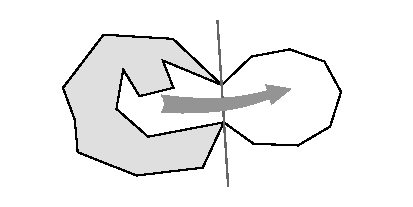
\includegraphics[scale=1.12]{img/carthage}
}
\end{tabular}\end{center}
\end{frame}